\documentclass[aspectratio=169]{beamer}

\usepackage[utf8]{inputenc}

\usepackage{amsmath}
\usepackage{graphicx}
\usepackage[T1]{fontenc}
\usepackage{Oswald}
\usepackage{array}

\usepackage{enumitem}
\setitemize{label=\usebeamerfont*{itemize item}%
  \usebeamercolor[fg]{itemize item}
  \usebeamertemplate{itemize item},
}
\setbeamertemplate{itemize item}[square]
\setbeamertemplate{itemize subitem}[circle]

\usepackage{pgfplots}
\pgfplotsset{compat=1.18}
\usepackage{tikz}
\usepgfplotslibrary{fillbetween}


% \tikzset{
% 	invisible/.style={opacity=0},
% 	visible on/.style={alt={#1{}{invisible}}},
% 	alt/.code args={<#1>#2#3}{%
% 		\alt<#1>{\pgfkeysalso{#2}}{\pgfkeysalso{#3}} % \pgfkeysalso doesn't change the path
% 	},
% }

%\pgfplotsset{every axis/.append style={label style={font=\small},tick label style={font=\footnotesize} }}

\newcommand{\graphheight}{7cm}
\newcommand{\graphwidth}{11cm}

\newcommand{\E}[1]{E\left[#1 \right]}
\newcommand{\ind}[1]{\mathbf{1}_{#1}}

%\newcommand{\P}[1]{E\left[#1\right]}

% \definecolor{azulcito}{RGB}{20,70,140}
\definecolor{azulcito}{RGB}{0,80,150}
\definecolor{verdecito}{RGB}{80,150,0}
\definecolor{rojito}{RGB}{150,0,80}
\definecolor{violetita}{RGB}{150,20,150}


\setbeamercolor*{structure}{fg=azulcito,bg=azulcito!20!white}
\setbeamercolor*{alerted text}{fg=azulcito}

  \setbeamercolor{block title}{fg=azulcito,bg=azulcito!20!white}
  \setbeamercolor{block body}{fg=black,bg=azulcito!10!white}
  
\beamertemplatenavigationsymbolsempty

\setbeamercolor*{author in head/foot}{fg=azulcito,bg=azulcito!15!white}
\setbeamercolor*{title in head/foot}{fg=azulcito,bg=azulcito!15!white}
\setbeamercolor*{date in head/foot}{fg=azulcito,bg=azulcito!15!white}

% Pgfplots
\pgfplotsset{width=\graphwidth, height = \graphheight, grid style = {dashed, gray}, every tick label/.append style = {font=\footnotesize}, compat=1.18, legend style={font=\footnotesize, draw=none, fill=none}, every axis/.append style={label style={font=\footnotesize}}}

\tikzset{>=stealth}

\newtheorem{proposition}{Proposition}

\defbeamertemplate*{footline}{mitema}
{
  \leavevmode%
  \hbox{%
  \begin{beamercolorbox}[wd=.25\paperwidth,ht=2.25ex,dp=1ex,left]{author in head/foot}%
    \usebeamerfont{author in head/foot}\hspace*{2ex}\insertshortauthor
  \end{beamercolorbox}%
  \begin{beamercolorbox}[wd=.5\paperwidth,ht=2.25ex,dp=1ex,center]{title in head/foot}%
    \usebeamerfont{date in head/foot}\insertshortdate{}
  \end{beamercolorbox}%
  \begin{beamercolorbox}[wd=.25\paperwidth,ht=2.25ex,dp=1ex,right]{date in head/foot}%
    \insertframenumber{}/\inserttotalframenumber\hspace*{2em} 
  \end{beamercolorbox}}%
 \vskip0pt%
}


\setbeamercolor{blocky}{fg=azulcito,bg=azulcito!15!white}
\setbeamercolor{blocky2}{fg=black,bg=azulcito!10!white}

\defbeamertemplate*{title page}{customized}[1][]
{
{\flushright
  \begin{beamercolorbox}[wd=\paperwidth,ht=6em,dp=1ex,right,rightskip=1.5em]{blocky}%
    \usebeamerfont{title}{\huge \inserttitle}\par \vspace{.9em}
    \usebeamerfont{subtitle}{\Large \insertsubtitle}\par \vspace{.5em}
  \end{beamercolorbox}%
  \vfill
    \usebeamerfont{author}{\Large \insertauthor}\par \vspace{1em}
      \usebeamerfont{institute}{\large \insertinstitute}\par
  
  
  \vfill
  \usebeamerfont{date}{\insertdate}\par
  %\usebeamercolor[fg]{titlegraphic}\inserttitlegraphic
  }
}

\usefonttheme[onlymath]{serif}

\title{The caching problem under a point process perspective}

\author[Andres Ferragut, Universidad ORT Uruguay]{Andres Ferragut\\[.6em] \normalsize joint work with Matias Carrasco and Fernando Paganini}
\institute{Universidad ORT Uruguay}
\date[Seminario PYE 2024]{Seminario PYE -- Universidad de la República -- Abril 2024}

\AtBeginSection[]
{
\begin{frame}{Outline}
\tableofcontents[currentsection, 
   hideallsubsections, 
   sectionstyle=show/shaded,
]
\end{frame}
}

\newenvironment*{myitem}[1][1.5em]{\begin{itemize}\setlength{\itemsep}{#1}}{\end{itemize}}

\begin{document}

\frame[plain]{\titlepage}

\begin{frame}{Outline}
\tableofcontents
\end{frame}

\section{The caching problem}

\begin{frame}{The caching problem}
	
	\begin{columns}
		\begin{column}{0.61\textwidth}
			\begin{myitem}[2em]
				\item Consider a \alert{cache system} with a catalog of $M$ objects.
				\item Requests for objects arrive at random.
				\item The cache can locally store $C<M$ of them.
				\item If item is in cache, we have a \alert{hit}. Otherwise, it is a \alert{miss}.
			\end{myitem}
		\end{column}
		\begin{column}{0.39\textwidth}
			\centering
			\input{figuras/cache_system.tikz}
		\end{column}
	\end{columns}

	\vfill

	\centering
	\alert{Objective:} for a given arrival stream, maximize the steady-state \alert{hit rate}.
\end{frame}

\begin{frame}{A sequential approach}

  \begin{myitem}
  \item Consider a sequence of random variables $Z_1,Z_2,\ldots$ with values in $\{1,\ldots,M\}$.
    
  \item Consider also the set:
   \begin{equation*}
    \mathcal{C} = \{\{i_1,\ldots,i_k\}\subset \{1,\ldots,M\}, k\leqslant C\} 
   \end{equation*}

  \item A (causal) caching policy would be a sequence of maps $\pi_n$ deciding which contents to store:
    \begin{equation*}
      \pi_n(Z_1,\ldots,Z_{n-1}) \to \mathcal{C}
    \end{equation*}

  \item In probabilistic terms, let $\mathcal{F}_n = \sigma(Z_1,\ldots,Z_n)$, then $\pi_n$ is any $\mathcal{C}-$valued $\mathcal{F}_n-$predictable process ($\mathcal{F}_{n-1}$-measurable).
  \end{myitem}


\end{frame}

\begin{frame}{A simple case}{The Independent Reference Model (IRM)}

  \begin{myitem}
    \item Assume now that $Z_n$ are $iid$ with distribution $p_i = P(Z_n=i)$, where $p_i$ is the \alert{popularity} of content $i$. Wlog, we take $p_1\geqslant p_2 \geqslant \ldots$.
    \item In this case, $Z_n\mid \mathcal{F}_{n-1} \sim p$, thus the hit probability at time $n$ is:
    \begin{equation*}
      P(Z_n \in \pi_n) = \E{\ind{Z_n\in\pi_n}} = \E{\E{\ind{Z_n\in \pi_n} \mid \mathcal{F}_{n-1}}} = \E{\sum_{i\in\pi_n} p_i} \leqslant \sum_{i=1}^C p_i
    \end{equation*}

    \item Taking $\pi_n \equiv \{1,\ldots,C\}$ achieves the bound.
    
  \end{myitem}
  \pause

  \vfill

  \alert{Conclusion:} under iid requests, the static ``keep the most popular'' policy is optimal.

\end{frame}

\begin{frame}{Practical policies: LFU and LRU}

  In practice, popularities are not known. This leads to the \alert{least-frequently-used (LFU)} eviction policy:
  \smallskip
  \begin{itemize}
    \item Take $\pi_n$ as the most requested objects so far (remove the least frequently used).
    \item In the long range, converges to the static policy.
  \end{itemize}

  \vfill

  Another popular eviction policy is \alert{least-recently-used (LRU)}, which treats $\pi_n$ as a list defined recursively:
  \smallskip
  \begin{itemize}
    \item If $Z_n \in \pi_n$, serve the content, move $Z_n$ to the front of the list.
    \item If $Z_n \notin \pi_n$, fetch the content, put $Z_n$ in the front of the list, remove the last object in the list (which is the least recently requested).
  \end{itemize}

\end{frame}

\begin{frame}{Beyond the IRM}

  \begin{myitem}[2em]

    \item Typically, requests are correlated, and popularities evolve over time.
    
    \item For instance, requests for a file may arrive in bursts.

    \item \alert{LRU} adapts to changes in popularity. Is good for bursts of requests. Tons of literature on this policy (also called move-to-front).

    \item However, performance metrics and optimality results are \alert{hard} to establish. 
  \end{myitem}
  
\end{frame}

\begin{frame}{The caching problem, take 2}

  Sequential models lack \alert{time information}, which may be useful!
  \pause
  \vfill

  \begin{block}{Point process approach [Fofack et al. 2014]:}

	
	\begin{itemize}
		\item Assume requests for item $i$ come from a \alert{point process} of intensity $\lambda_i := \lambda p_i$.

    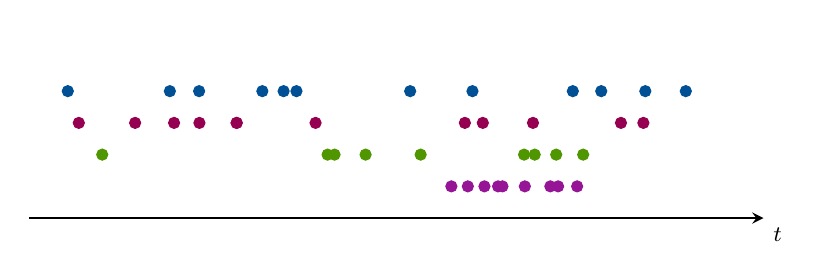
\begin{tikzpicture}
			\begin{axis}[
        width=0.9\columnwidth,
				xlabel=$t$,
				ymin = 0,
				ymax = .6,
				xmin = 0,
				xmax=22,
				xlabel style = {at={(axis cs:22,0)},anchor=north west},
				y axis line style={draw=none},
				x axis line style={->, thick},
				ticks=none,
				axis x line*=middle,
				height=4cm,
				]
			\addplot+[azulcito, mark options={fill=azulcito},mark=*,only marks] coordinates {
				(1.168317969682793,0.4)
				(4.224371806575089,0.4)
				(5.099828260436964,0.4)
				(6.9938720827411025,0.4)
				(7.629926439960695,0.4)
				(8.015139525296764,0.4)
				(11.41978663218779,0.4)
				(13.285132721106107,0.4)
				(16.28953436494327,0.4)
				(17.14081344555717,0.4)
				(18.46073553951872,0.4)
				(19.6728937320483,0.4)
			};
			\addplot+[rojito, mark options={fill=rojito},mark=*,only marks] coordinates {
				(1.49783995292964,.3)
  				(3.184138404294451,.3)
  				(4.35051050123616,.3)
  				(5.1091887517481505,.3)
  				(6.221541171374557,.3)
  				(6.226859317209702,.3)
  				(8.586778366165495,.3)
				(13.057655264423126,.3)
 				(13.594421727013588,.3)
 				(15.096680803679005,.3)
				(17.731518813017008,.3)
 				(18.40246895328477,.3)				
			};
      \addplot+[verdecito, mark options={fill=verdecito}, mark=*,only marks] coordinates {
				(2.1995364349536235,0.2)
				(8.947058606859512,0.2)
  				(9.155089124125874,0.2)
 				(10.084686662202682,0.2)
 				(11.733424911823171,0.2)
 				(14.830631279727431,0.2)
 				(15.149252788554351,0.2)
 				(15.791821681936792,0.2)
 				(16.599742636184,0.2)

			};
			\addplot+[violetita,mark options={fill=violetita},mark=*,only marks] coordinates {
				(12.653556737204989,0.1)
 				(13.146127585840045,0.1)
 				(13.643536674608884,0.1)
 				(14.051631664505377,0.1)
 				(14.183143031766923,0.1)
 				(14.85305783374829,0.1)
 				(15.61726438611725,0.1)
 				(15.848820745581179,0.1)
 				(16.419089799482926,0.1)
			};
			\end{axis}
		\end{tikzpicture}

		\item At each point in time we must decide which items must be stored locally.
	\end{itemize}
\end{block}

If inter-request times are \alert{heavy tailed}, this can model burstiness.
\end{frame}

\begin{frame}{Example: Pareto arrivals}

	Consider two items, with equal popularity...

	\vfill

	\begin{myitem}[1em]
		\item Poisson arrivals:
		
		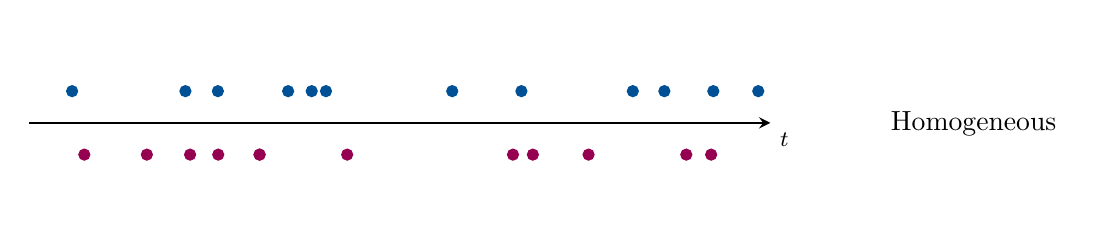
\begin{tikzpicture}
			\begin{axis}[
				xlabel=$t$,
				ymin = -.3,
				ymax = .3,
				xmin = 0,
				xmax=20,
				xlabel style = {at={(axis cs:20,0)},anchor=north west},
				y axis line style={draw=none},
				x axis line style={->, thick},
				ticks=none,
				axis x line*=middle,
				height=4cm,
				]
			\addplot+[azulcito, mark options={fill=azulcito},mark=*,only marks] coordinates {
				(1.168317969682793,0.1)
				(4.224371806575089,0.1)
				(5.099828260436964,0.1)
				(6.9938720827411025,0.1)
				(7.629926439960695,0.1)
				(8.015139525296764,0.1)
				(11.41978663218779,0.1)
				(13.285132721106107,0.1)
				(16.28953436494327,0.1)
				(17.14081344555717,0.1)
				(18.46073553951872,0.1)
				(19.6728937320483,0.1)
			};
			\addplot+[rojito, mark options={fill=rojito},mark=*,only marks] coordinates {
				(1.49783995292964,-.1)
  				(3.184138404294451,-.1)
  				(4.35051050123616,-.1)
  				(5.1091887517481505,-.1)
  				(6.221541171374557,-.1)
  				(6.226859317209702,-.1)
  				(8.586778366165495,-.1)
				(13.057655264423126,-.1)
 				(13.594421727013588,-.1)
 				(15.096680803679005,-.1)
				(17.731518813017008,-.1)
 				(18.40246895328477,-.1)				
			};
			\end{axis}
			\node at (12,1.2) {Homogeneous};
		\end{tikzpicture}

		\item Heavy tailed arrivals (Pareto $\alpha=2$):
		
		\begin{tikzpicture}
			\begin{axis}[
				xlabel=$t$,
				ymin = -.3,
				ymax = .3,
				xmin = 0,
				xmax=20,
				xlabel style = {at={(axis cs:20,0)},anchor=north west},
				y axis line style={draw=none},
				x axis line style={->, thick},
				ticks=none,
				axis x line*=middle,
				height=4cm,
				]
			\addplot+[azulcito, mark options={fill=azulcito}, mark=*,only marks] coordinates {
				(2.1995364349536235,.1)
				(8.947058606859512,.1)
  				(9.155089124125874,.1)
 				(10.084686662202682,.1)
 				(11.733424911823171,.1)
 				(14.830631279727431,.1)
 				(15.149252788554351,.1)
 				(15.791821681936792,.1)
 				(16.599742636184,.1)

			};
			\addplot+[rojito,mark options={fill=rojito},mark=*,only marks] coordinates {
				(12.653556737204989,-.1)
 				(13.146127585840045,-.1)
 				(13.643536674608884,-.1)
 				(14.051631664505377,-.1)
 				(14.183143031766923,-.1)
 				(14.85305783374829,-.1)
 				(15.61726438611725,-.1)
 				(15.848820745581179,-.1)
 				(16.419089799482926,-.1)
			};
			\end{axis}
			\node at (12,1.2) {Bursty!};
		\end{tikzpicture}

	\end{myitem}

\end{frame}

\begin{frame}{Some open questions...}

  \begin{myitem}[2em]

    \item What is the optimal causal policy in this framework?
    
    \item Can we compute the optimal hit rate/hit probability?
    
    \item What is its large scale behavior?
    
    \item How typical policies compare to the optimal one?
  \end{myitem}

\end{frame}
\section{Point processes and stochastic intensity}

\begin{frame}{A bit of point process theory...}
	
	Let $N = \{T_k:k\in\mathbb{Z}\}$ be a \alert{stationary point process} representing request times:

	\begin{center}

	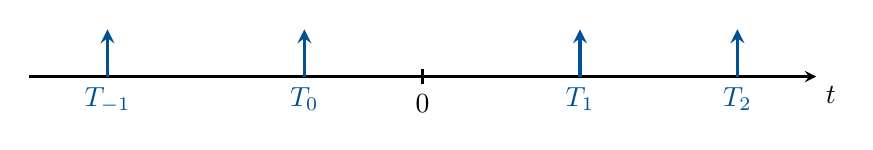
\begin{tikzpicture}
	   
		\draw[->,thick] (-5,0) -- (5,0);
		\node[below right] at (5,0) {$t$};
		
		\draw[<-,very thick, azulcito] (-4,.6) -- (-4,0) node[below] {$T_{-1}$};
		\draw[<-,very thick, azulcito] (-1.5,.6) -- (-1.5,0) node[below] {$T_{0}$};
		\draw[<-,very thick, azulcito] (2,.6) -- (2,0) node[below] {$T_{1}$};
		\draw[<-,very thick, azulcito] (4,.6) -- (4,0) node[below] {$T_{2}$};
		\draw[-,thick] (0,-.1) node[below] {$0$} -- (0,0.1);
		 
		% \draw<2->[->, very thick, verdecito] (1,.4) -- node[midway, above, anchor=south] {$X\sim F$} (4,.4);

		% \draw<3->[->, very thick, rojito] (8,.4) -- node[midway, above, anchor=south] {$\hat{X}\sim \hat{F}$} (6,.4);

	\end{tikzpicture}

	\end{center}
	i.e. $N(B) = \sum_n \ind{\{T_n\in B\}}$ is a \emph{random counting measure}.

	\pause \vfill

	\begin{columns}
		\begin{column}{0.4\textwidth}
			\alert{Counting process:}
			\begin{equation*}
				N(t) = \begin{cases}
					N([0,t]) & t\geqslant 0 \\
					-N((t,0)) & t<0
				\end{cases}
			\end{equation*}
		\end{column}
		\begin{column}{0.6\textwidth}
			\begin{tikzpicture}
				\begin{axis}[
					width=\columnwidth,
					height= 0.5\columnwidth,
					xlabel=$t$,
					ymin = -2.1,
					ymax = 2.1,
					xmin = -5,
					xmax=5,
					xlabel style = {at={(axis cs:7,0)},anchor=north west},
					y axis line style={draw=none},
					x axis line style={->, thick},
					xtick={0},
					ymajorticks=false,
					axis x line*=middle,
					]
		
					\addplot+[azulcito, mark options={fill=azulcito, scale=1.5}, mark=*,only marks] coordinates {
						(-4,0)
						(-1.5,0)
						(2,0)
						(4,0)
					};
					\addplot+[rojito, const plot, no marks, very thick] coordinates {
						(-5,-2)
						(-4,-1)
						(-1.5,-0)
						(2,1)
						(4,2)
						(5,2)
					};
					\node[above left, rojito] at (axis cs:4,1) {$N(t)$};
				\end{axis}
			\end{tikzpicture}
		\end{column}
	\end{columns}
	\pause \vfill

	Let $\mathcal{F}_t = \sigma(N(s), s\leqslant t)$ be its \alert{internal history}.
\end{frame}

	\begin{frame}{Two important distributions:}

		\begin{center}

			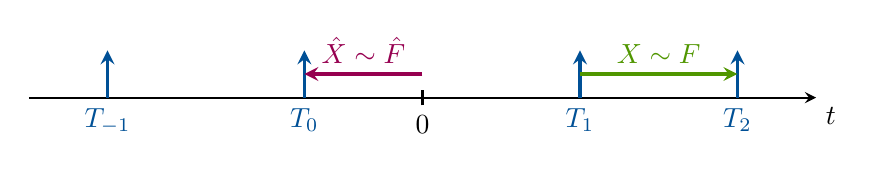
\begin{tikzpicture}
			   
				\draw[->,thick] (-5,0) -- (5,0);
				\node[below right] at (5,0) {$t$};
				
				\draw[<-,very thick, azulcito] (-4,.6) -- (-4,0) node[below] {$T_{-1}$};
				\draw[<-,very thick, azulcito] (-1.5,.6) -- (-1.5,0) node[below] {$T_{0}$};
				\draw[<-,very thick, azulcito] (2,.6) -- (2,0) node[below] {$T_{1}$};
				\draw[<-,very thick, azulcito] (4,.6) -- (4,0) node[below] {$T_{2}$};
				\draw[-,thick] (0,-.1) node[below] {$0$} -- (0,0.1);
				 
				\draw[->, very thick, verdecito] (2,.3) -- node[midway, above, anchor=south] {$X\sim F$} (4,.3);
		
				\draw<2->[->, very thick, rojito] (0,.3) -- node[midway, above, anchor=south] {$\hat{X}\sim \hat{F}$} (-1.5,.3);
		
			\end{tikzpicture}
		
		\end{center}

		\vfill

		\begin{tabular}{m{4cm} m{6cm}}
			\alert{Inter-arrival distribution:} & 
					\begin{gather*}
						F(t) := P^0_N (T_1 - T_0 \leqslant t), \quad
						E^0_N[T_1] = 1/\lambda.
					\end{gather*} \\[-2em]
					\uncover<2->{
			\alert{Age distribution:} &
					\begin{equation*}
						\hat{F}(t) := P (- T_0 \leqslant t) = \lambda \int_0^t 1-F(s)ds,
					\end{equation*}}
		\end{tabular}
			\vfill

		Note: here $P^0_N$ is the \alert{Palm probability} of the point process (conditioning on $T_0=0$).

\end{frame}

\begin{frame}{Stochastic intensity}
	Consider a simple stationary point process $N$ with intensity $\lambda$, defined in some probability space $(\Omega, \mathcal{F},P)$. Let some filtration $\{\mathcal{F}_t\}_{t\in\mathbb{R}}$ be a \alert{history} of the process.

	\bigskip

	\begin{block}{Definition:}

		The random process $\lambda(t)\geqslant 0$ is a \alert{stochastic intensity} for the history $\mathcal{F}_t$ iff it is a.s. locally integrable, $\mathcal{F}_t-$adapted and:
		\begin{equation*}
			\E{N((a,b])\mid \mathcal{F}_a} = \E{\left.\int_a^b \lambda(t)dt \right| \mathcal{F}_a}
		\end{equation*}
		for all $a,b\in \mathbb{R}$.
	\end{block}

\end{frame}

\begin{frame}{Stochastic intensity}{Properties}

	
	\alert{Local interpretation:}
		\begin{equation*}
			E[N((t,t+h])\mid \mathcal{F}_t] = \lambda(t)h + o(h) \quad P-a.s.,
		\end{equation*}
	
	So $\lambda(t)$ acts as a \alert{local} notion of intensity based on previous history.

	\pause \vfill
	\alert{Martingale interpretation:}
		\begin{equation*}
			M_a(t) = N(t) - N(a) - \int_a^t \lambda(s)ds
		\end{equation*} 
		is a local $(P,\mathcal{F}_t)$ martingale for any $a\in\mathbb{R}$.
	
		\vfill

	Namely, $A(t) = N(a) + \int_a^t \lambda(s)ds$ is the \alert{compensator} of the counting process.

\end{frame}

\begin{frame}{Stochastic intensity of a Poisson process}

	\begin{myitem}[2em]
		\item If $N(t)$ is a Poisson process, then we know that
		\begin{equation*}
			M(t) = N(t) - \lambda t = N(t) - \int_0^t \lambda dt
		\end{equation*}
		is a martingale, so the stochastic intensity of a Poisson process is just $\lambda(t)\equiv \lambda$.

		\pause

		\item In fact, this \alert{characterizes} the Poisson process. The stochastic intensity $\lambda(t)$ is \alert{deterministic} if and only if $N$ is a Poisson process of (possible time-varying) intensity $\lambda(t)$.
	\end{myitem}
\end{frame}

\begin{frame}{Stochastic intensity}{A local notion of intensity...}
	
	However, if traffic is \alert{bursty}, the stochastic intensity \alert{rises} after arrivals:

	\vfill

	\begin{center}
	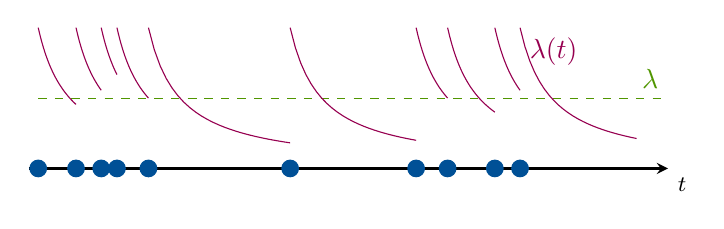
\begin{tikzpicture}
		\begin{axis}[xlabel=$t$,
			ymin = -.3,
			ymax = 2,
			xmin = -.3,
			xmax=20,
			xlabel style = {at={(axis cs:20,0)},anchor=north west},
			y axis line style={draw=none},
			x axis line style={->, thick},
			ticks=none,
			axis x line*=middle,
			width=0.8\textwidth,
			height= 0.3\textwidth,
			]
			\addplot[verdecito,domain=0:20, dashed] {1};
			\addplot[rojito,domain=0:1.2] {2/(1+x)};
			\addplot[rojito,domain=1.2:2] {2/(1+x-1.2)};
			\addplot[rojito,domain=2:2.5] {2/(1+x-2)};
			\addplot[rojito,domain=2.5:3.5] {2/(1+x-2.5)};
			\addplot[rojito,domain=3.5:8] {2/(1+x-3.5)};
			\addplot[rojito,domain=8:12] {2/(1+x-8)};
			\addplot[rojito,domain=12:13] {2/(1+x-12)};
			\addplot[rojito,domain=13:14.5] {2/(1+x-13)};
			\addplot[rojito,domain=14.5:15.3] {2/(1+x-14.5)};
			\addplot[rojito,domain=15.3:19] {2/(1+x-15.3)};
			\node[below right, rojito] at (axis cs:15.3,2) {$\lambda(t)$};
			\node[above left, verdecito] at (axis cs:20,1) {$\lambda$};

			\addplot+[azulcito, mark options={fill=azulcito, scale=1.5}, mark=*,only marks] coordinates {
				(0,0)
				(1.2,0)
 				(2,0)
 				(2.5,0)
 				(3.5,0)
 				(8,0)
 				(12,0)
 				(13,0)
 				(14.5,0)
 				(15.3,0)
			};
		\end{axis}
	\end{tikzpicture}
	\end{center}

	\vfill
	Note: for stationary processes, $E[\lambda(t)] = E[\lambda(0)] = \lambda$, the average intensity.
\end{frame}

\begin{frame}{Renewal processes}

	\begin{itemize}
	\item Let now $N$ be a \alert{stationary renewal process}, i.e. inter request times $T_{n+1}-T_n$ are $iid\sim F$.
	
	\item Assume that $F$ has a density, and define the \alert{hazard rate} of $F$ as:
	 \begin{equation*}
		\eta(t) = \frac{f(t)}{1-F(t)}
	 \end{equation*}

	\end{itemize}
	\pause
	 \begin{theorem}[Daley-Vere Jones, Chapter 7]
		For a renewal process and its natural history, the stochastic intensity is:
		\begin{equation*}
			\lambda(t) = \eta(t-T^*(t)),
		\end{equation*}
		where 
		\begin{equation*}
			T^*(t) = \sup\{T_n:T_n<t\}
		\end{equation*}
		is the last point before $t$.
	\end{theorem}

\end{frame}

\begin{frame}{Some examples...}

	\begin{tabular}{m{7cm} m{6cm}}

		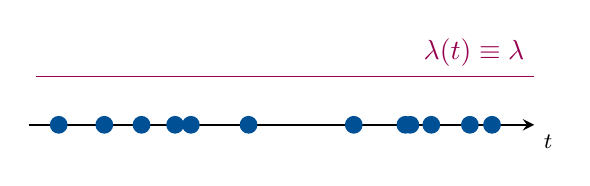
\begin{tikzpicture}
			\begin{axis}[xlabel=$t$,
				ymin = -.3,
				ymax = 2,
				xmin = -.3,
				xmax=20,
				xlabel style = {at={(axis cs:20,0)},anchor=north west},
				y axis line style={draw=none},
				x axis line style={->, thick},
				ticks=none,
				axis x line*=middle,
				width=8cm,
				height= 3cm,
				]
				\addplot[rojito, domain=0:20] {1};
				\node[above left, rojito] at (axis cs:20,1) {$\lambda(t)\equiv \lambda$};
	
				\addplot+[azulcito, mark options={fill=azulcito, scale=1.5}, mark=*,only marks] coordinates {
					(0.9028581008067987,0)
					(2.7341797790213573,0)
					(4.228330726726128,0)
					(5.577074925845067,0)
					(6.211423990911654,0)
					(8.528255357570485,0)
					(12.753859672976413,0)
					(14.826517141978712,0)
					(15.028110470502309,0)
					(15.868264106338712,0)
					(17.418133532477547,0)
					(18.306210880027027,0)
				};
			\end{axis}
		\end{tikzpicture} & \alert{Constant hazard rate} $\to$ Poisson process.\\
		\\
		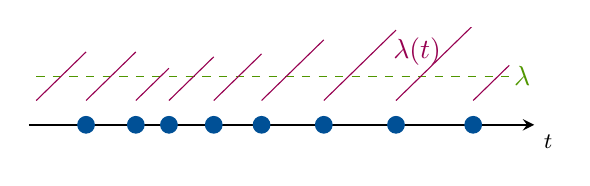
\begin{tikzpicture}
			\begin{axis}[xlabel=$t$,
				ymin = -.3,
				ymax = 2,
				xmin = -.3,
				xmax=20,
				xlabel style = {at={(axis cs:20,0)},anchor=north west},
				y axis line style={draw=none},
				x axis line style={->, thick},
				ticks=none,
				axis x line*=middle,
				width=8cm,
				height=3cm,
				]
				\addplot[verdecito,domain=0:19, dashed] {1};
				\addplot[rojito,domain=0:2] {0.5+0.5*x};
				\addplot[rojito,domain=2:4] {0.5+0.5*(x-2};
				\addplot[rojito,domain=4:5.33] {0.5+0.5*(x-4};
				\addplot[rojito,domain=5.33:7.13] {0.5+0.5*(x-5.33};
				\addplot[rojito,domain=7.13:9.05] {0.5+0.5*(x-7.13};
				\addplot[rojito,domain=9.05:11.55] {0.5+0.5*(x-9.05};
				\addplot[rojito,domain=11.55:14.45] {0.5+0.5*(x-11.55};
				\addplot[rojito,domain=14.45:17.55] {0.5+0.5*(x-14.45};
				\addplot[rojito,domain=17.55:19] {0.5+0.5*(x-17.55};
				\node[below, rojito] at (axis cs:15.3,2) {$\lambda(t)$};
				\node[right, verdecito] at (axis cs:18.8,1) {$\lambda$};

				\addplot+[azulcito, mark options={fill=azulcito, scale=1.5}, mark=*,only marks] coordinates {
					(2,0)
					(4,0)
					(5.33,0)
					(7.13,0)
					(9.05,0)
					(11.55,0)
					(14.45,0)
					(17.55,0)
				};
			\end{axis}
		\end{tikzpicture} & \alert{Increasing} hazard rate $\to$ more periodic!\\
		\\
		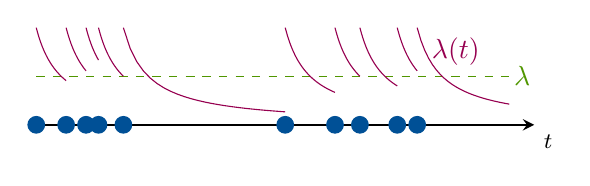
\begin{tikzpicture}
			\begin{axis}[xlabel=$t$,
				ymin = -.3,
				ymax = 2,
				xmin = -.3,
				xmax=20,
				xlabel style = {at={(axis cs:20,0)},anchor=north west},
				y axis line style={draw=none},
				x axis line style={->, thick},
				ticks=none,
				axis x line*=middle,
				width=8cm,
				height=3cm,
				]
				\addplot[verdecito,domain=0:19, dashed] {1};
				\addplot[rojito,domain=0:1.2] {2/(1+x)};
				\addplot[rojito,domain=1.2:2] {2/(1+x-1.2)};
				\addplot[rojito,domain=2:2.5] {2/(1+x-2)};
				\addplot[rojito,domain=2.5:3.5] {2/(1+x-2.5)};
				\addplot[rojito,domain=3.5:10] {2/(1+x-3.5)};
				\addplot[rojito,domain=10:12] {2/(1+x-10)};
				\addplot[rojito,domain=12:13] {2/(1+x-12)};
				\addplot[rojito,domain=13:14.5] {2/(1+x-13)};
				\addplot[rojito,domain=14.5:15.3] {2/(1+x-14.5)};
				\addplot[rojito,domain=15.3:19] {2/(1+x-15.3)};
				\node[below right, rojito] at (axis cs:15.5,2) {$\lambda(t)$};
				\node[right, verdecito] at (axis cs:18.8,1) {$\lambda$};
	
				\addplot+[azulcito, mark options={fill=azulcito, scale=1.5}, mark=*,only marks] coordinates {
					(0,0)
					(1.2,0)
					 (2,0)
					 (2.5,0)
					 (3.5,0)
					 (10,0)
					 (12,0)
					 (13,0)
					 (14.5,0)
					 (15.3,0)
				};
			\end{axis}
		\end{tikzpicture} & \alert{Decreasing} hazard rate $\to$ more bursty!


	\end{tabular}
\end{frame}


\section{The optimal caching policy}

\begin{frame}{The predictable $\sigma-$algebra}

	Let $(\Omega,\mathcal{F},\{\mathcal{F}_t: t\in\mathbb{R}\},P)$ be a filtered probability space.

	\bigskip

	\begin{definition}
		The predictable $\sigma-$algebra $\mathcal{P}(\mathcal{F}.)$ is the $\sigma-$álgebra in $\mathbb{R}\times \Omega$ generated by the sets:
		\begin{equation*}
			(a,b] \times A, \; a<b, \; A\in\mathcal{F}_a, 
		\end{equation*}
	\end{definition}

\end{frame}

\begin{frame}{Predictable processes}

	\begin{definition}[Predictable process]
		A stochastic process $X(t,\omega)$ taking values on a measurable space $(E,\mathcal{E})$ is \alert{$\mathcal{F}_t-$predictable} if the mapping $(t,\omega) \mapsto X(t,\omega)$ is $\mathcal{P}(\mathcal{F}.)-$measurable.
	\end{definition}

	\vfill
	\begin{myitem}
		\item \alert{Key idea:} a process is $\mathcal{F}_t-$predictable if its value at $t$ is completely determined by the information prior to $t$.
		\pause
		\item In particular $\mathcal{F}_t-$adapted $+$ left continuous $\Longrightarrow$ $\mathcal{F}_t$-predictable.
		
		\item Since the stochastic intensity of a point process can be chosen left-continuous, it is $\mathcal{F}_t$-predictable.
	\end{myitem}

\end{frame}
\begin{frame}{Causal caching policies}
	
	\begin{myitem}[1em]
		\item Consider again a cache system fed by $M$ \alert{independent} request processes $N_i(t)$ with stochastic intensities $\lambda_i(t)$.
		\item Let $\mathcal{F}_t = \sigma(\{\mathcal{F}_t^{(i)}: i=1,\ldots,M\})$ their aggregate history.
	\end{myitem}

	\vfill

	\begin{block}{Definition}
		A \alert{causal} caching policy is an $\mathcal{F}_t$ \alert{predictable} stochastic process
		\begin{equation*}
			\pi(t):\Omega\times\mathbb{R} \to \mathcal{C}
		\end{equation*}
		i.e. $\pi(t) = \{i_1,\ldots,i_k\}$ (with $k\leqslant C$) is the subset kept at time $t$, and only depends on the past history of item requests.
	\end{block}

\end{frame}

\begin{frame}{The hit process}{Stochastic intensity}
	
	Focus now on a particular content $i$, its \alert{hit process} is the point process given by:

	\vfill

	\begin{columns}
		\begin{column}{0.5\textwidth}
			\begin{equation*}
				H_i(B) = \sum_{n\in\mathbb{Z}} \ind{\{T_n^i\in B\}}\ind{\{i\in \pi(T_n^i)\}}
			\end{equation*}
		\end{column}
		\begin{column}{0.5\textwidth}
			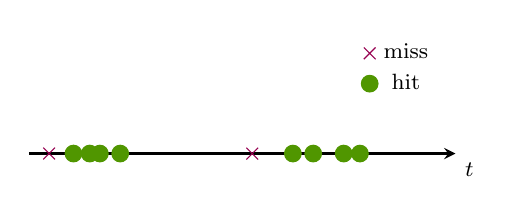
\begin{tikzpicture}
				\begin{axis}[xlabel=$t$,
					ymin = -.3,
					ymax = 1.5,
					xmin = -1,
					xmax=20,
					xlabel style = {at={(axis cs:20,0)},anchor=north west},
					y axis line style={draw=none},
					x axis line style={->, thick},
					ticks=none,
					axis x line*=middle,
					width=7cm,
					height=3.5cm,
					legend pos=north east
					]
					\addplot+[rojito, mark options={fill=rojito, scale=1.5}, mark=x,only marks] coordinates {
						(0,0)
						 (10,0)
					};
					\addlegendentry{miss}
					\addplot+[verdecito, mark options={fill=verdecito, scale=1.5}, mark=*,only marks] coordinates {
						(1.2,0)
						 (2,0)
						 (2.5,0)
						 (3.5,0)
						 (12,0)
						 (13,0)
						 (14.5,0)
						 (15.3,0)
					};
					\addlegendentry{hit}
				\end{axis}
			\end{tikzpicture}

		\end{column}
	\end{columns}

	\vfill

	Now $\ind{\{i\in \pi(t)\}}$ is $\mathcal{F}_t$-predictable, so the stochastic intensity of $H_i$ is:
	\begin{equation*}
		h_i(t) = \lambda_i(t) \ind{\{i\in \pi(t)\}}
	\end{equation*}
	i.e., $h_i(t)=\lambda_i(t)$ while $i$ is cached and otherwise $0$.
\end{frame}

\begin{frame}{The hit process}{The hit rate}
	If we now consider the aggregate of requests, the \alert{total hit process} is given by:
	\begin{equation*}
		H = \sum_{i=1}^M H_i
	\end{equation*}

	And its stochastic intensity is just:
	\begin{equation*}
		h(t) = \sum_{i=1}^M h_i(t) = \sum_{i=1}^M \lambda_i(t) \ind{\{i\in \pi(t)\}}
	\end{equation*}

	The steady state \alert{hit rate} of the policy is:
	\begin{equation*}
		\text{hit rate} = \lambda_{\text{hit}} := E[h(t)]
	\end{equation*}
	
\end{frame}

\begin{frame}{Maximizing the hit rate}
	
	In order to maximize $\lambda_{\text{hit}}$, consider the causal policy:
	\begin{equation*}
		\pi^*(t) = \{i_1,\ldots,i_C\} \quad \text{such that}\; \sum_{i\in\{i_1,\ldots,i_C\}} \lambda_{i}(t) \text{ is maximized.}
	\end{equation*}

	Then, for any causal policy $\pi$ and for each realization:
	\begin{equation*}
		h(t) = \sum_{i\in\pi(t)} \lambda_i(t) \leqslant \sum_{i\in \pi^*(t)} \lambda_i(t) = h^*(t).
	\end{equation*} 

	\begin{theorem}
		The \alert{optimal causal policy} is to keep in the cache the $C$ objects with the \alert{highest stochastic intensity} at any time.
	\end{theorem}

\end{frame}

\begin{frame}{Back to the Poisson case}

	\begin{myitem}
		\item Assume the $N_i$ are Poisson processes of intensities $\lambda_i$.
		\item We take $\lambda_1>\lambda_2>\ldots$ as the popularities.
		\item The total request process is also Poisson of intensity $\sum_i\lambda_i$.
		\item In that case, the optimal policy is:
		\begin{equation*}
			\pi^*(t) \equiv \{1,\ldots,C\}
		\end{equation*}
		since $\lambda_i(t)\equiv \lambda_i$ and these are is decreasing.
	\end{myitem}

	\pause \vfill
	\alert{Conclusion:} under Poisson arrivals, statically keeping the most popular objects is optimal (compare to the IRM before).
\end{frame}

\begin{frame}{The renewal case}
	\begin{myitem}[2em]
		\item If now the $N_i$ are renewal processes of (decreasing) intensities $\lambda_i$.
		\item The total request process is no longer renewal, but its intensity is again $\sum_i\lambda_i$.
		\item Since $\lambda_i(t) = \eta_i(t-T^*_i(t))$, the optimal policy is:
		\vspace{1em}
		\begin{itemize}
			\item Keep track of the \alert{current hazard rate} of each content $i$.
			\vspace{.5em}
			\item Choose to keep in $\pi^*(t)$ the $C$ highest. 
		\end{itemize}
	\end{myitem}

	\pause \vfill
	\alert{Conclusion:} under renewal arrivals, the optimal policy only depends on the current hazard rates since the last request.
\end{frame}

\begin{frame}{An interesting observation}

	\alert{Decreasing hazard rates}

	\begin{myitem}[1em]
		\item If hazard rates are \alert{decreasing}, caching makes sense! After an arrival it becomes more likely to get another request.
		\item After some time, we will evict the content to make room for more recent ones (as in LRU).
	\end{myitem}

	\pause\vfill
	\alert{Increasing hazard rates}

	\begin{myitem}[1em]
		\item If instead hazard rates are \alert{increasing}, then when a request arrives, the item becomes less likely to be requested again! 
		\item It may be better to remove it and make room for other ones (i.e. LRU makes no sense!).
		\item If we haven't seen it for a while, then we may have to fetch it \alert{anticipating} the upcoming request.
	\end{myitem}
\end{frame}

\section{Large scale asymptotics}

\begin{frame}{Understanding the optimal policy}{The threshold process}
	
	We can rewrite this optimal policy as a \alert{threshold} policy:

	\begin{equation*}
		i\in\pi^*(t) \Leftrightarrow \lambda_i(t) \geqslant \theta(t) := \text{ the $C$ largest stochastic intensity}
	\end{equation*}

	\vfill
	\alert{Example:} Pareto requests, Zipf popularities, $N=20, C=4$.
	\begin{center}
		\input{figuras/threshold_process.tikz}
	\end{center}

	\vfill

	¿What is the large scale behavior of $\theta(t)$ in steady state?.
\end{frame}

% \begin{frame}{A useful lemma}
	
% 	\begin{columns}
% 		\begin{column}{0.5\textwidth}
% 			What's the stochastic intensity \alert{distribution} in steady state?			
% 		\end{column}
% 		\begin{column}{0.5\textwidth}
% 			\begin{tikzpicture}
% 				\begin{axis}[xlabel=$t$,
% 					ymin = -2,
% 					ymax = 3,
% 					xmin = -.3,
% 					xmax = 4.5,
% 					xlabel style = {at={(axis cs:4.5,0)},anchor=north west},
% 					y axis line style={draw=none},
% 					x axis line style={->, thick},
% 					ytick=\empty,
% 					axis x line*=middle,
% 					axis y line*=left,
% 					width=7.5cm,
% 					height=5cm,
% 					xtick={0,4},
% 					ytick={.8},
% 					xticklabels={$\tau_0$,$\tau_1$},
% 					yticklabels={$x$},
% 					]
% 					\addplot[domain=0:4,thick,azulcito] {2/(1+x)} node[midway, yshift=10, xshift=3,anchor=south east]{$\eta(t-\tau_0)$};
% 					\addplot[domain=0:4,dashed] {0.8};
% 					\fill[color=azulcito, opacity=0.1] (1.5,0) rectangle (4,0.8);
% 					\draw [verdecito,decoration={brace,mirror,raise=0.5cm},decorate] (axis cs:0,0) -- (axis cs:4,0) node [pos=0.5,anchor=north,yshift=-0.55cm] {Cycle $\approx 1/\lambda$}; 
% 					\draw [rojito,decoration={brace,raise=0.05cm},decorate] (axis cs:1.5,.8) -- (axis cs:4,0.8) node [pos=0.5,anchor=south,yshift=0.1cm] {$\mathbf{1}_{\{\eta(s)<x\}}$};
% 				\end{axis}
% 			\end{tikzpicture}
% 		\end{column}
% 	\end{columns}
% 	\vfill
% 	\begin{lemma}
% 		If requests come from a Pareto($\alpha$) renewal process, with intensity $\lambda$, from the master equation:
% 		\begin{equation*}
% 			P(\lambda(0)\leqslant x) = \lambda E^0_{N}\left[\int_0^{\tau_1}\mathbf{1}_{\{\eta(s)\leqslant x\}}ds\right] = \left(\frac{\theta x}{\alpha}\right)^{\alpha-1}, \quad 0\leqslant x \leqslant \alpha/\theta,
% 		\end{equation*}
% 		with $\theta = (\alpha-1)/\lambda$.
% 	\end{lemma}
% \end{frame}

	

\begin{frame}{The threshold value in steady state}
	
	\begin{myitem}[1em]
		\item Now we have $M$ independent renewal processes with intensities $\lambda_i(t)$.
		\item At time $t=0$, we have a sample $\{X_1,\ldots,X_M\}$ of independent, but \textbf{not identically distributed} random variables, with distribution:
		\begin{equation*}
			X_i \sim \eta_i(-T_0^i), \quad -T_0\sim \hat{F}_i(t) 
		\end{equation*}

		\item The threshold $\theta(0)$ is the $C-$th \alert{order statistic} (in decreasing order) of the sample.
	\end{myitem}
	\vfill
	\alert{Problem:} for non $iid$ random variables, no closed form $\to$ Can we say something about the large scale limit?
\end{frame}

\begin{frame}{A useful Theorem}
	
	Let $\{X_i\}$ be a sequence of independent random variables with distributions $G_i$. Define:
	\begin{equation*}
		\hat{G}_M(x) = \frac{1}{M}\sum_{i=1}^M \ind{\{X_i\leqslant x\}}
	\end{equation*}
	the empirical distribution, and let:
	\begin{equation*}
		\bar{G}_M(x) = \frac{1}{M}\sum_{i=1}^M G_i(x)
	\end{equation*}
	
	\begin{theorem}[Shorack]
		If the family $\{G_i\}$ is tight, then:
		\begin{equation*}
			||\hat{G}_M - \bar{G}_M||_\infty \to 0 \quad \text{almost surely as }M\to\infty.
		\end{equation*}
	\end{theorem}
\end{frame}

\begin{frame}{Back to caching...}{A little more structure}
	
	Assume now that the request processes come from a common scale family, i.e. their inter-arrival distributions satisfy:
	\begin{equation*}
		F_i(t) = F_0(\lambda_i t)
	\end{equation*}
	where $F_0$ has mean $1$, so $F_i$ has mean $1/\lambda_i$.

	\pause \vfill

	In this case:
	\begin{myitem}[1em]
		\item The distribution of $-T_0^i$ is $\hat{F}_i(t) = \hat{F}_0(\lambda_i t)$.
		\item The hazard-rate of $F_i$ is $\eta_i(t) = \lambda_i \eta_0(t/\lambda_i)$.
		\item The random variable $X_i\sim G_i(x):=G_0(x/\lambda_i)$
	\end{myitem}
	\vfill
	where $G_0(x) = P(\eta_0(-T_0)\leqslant x)$ is the observed hazard rate distribution for the base process.

\end{frame}

\begin{frame}{The distribution of popularities}
	
	Consider now the popularities $\lambda_1> \ldots > \lambda_M$ and define:
	\begin{equation*}
		\phi_M(\lambda) = \frac{1}{M}\sum_{i=1}^M \ind{\{\lambda_i\leqslant \lambda\}}
	\end{equation*}
	their empirical (deterministic) distribution.

	\pause \vfill
	\alert{Assumption:}
	\begin{equation*}
		\phi_M(\lambda) \to \phi(\lambda) \quad \text{as } M\to\infty
	\end{equation*}
	where $\phi(\lambda)$ is a probability distribution.
\end{frame}

\begin{frame}{Example: Zipf popularities}
	
	\begin{myitem}
		\item A common model for popularities is the \alert{Zipf} distribution, where $\lambda_i \propto \frac{1}{i^\beta}$.
		\item In our framework, take:
			\begin{equation*}
				\lambda_i = \left(\frac{M}{i}\right)^\beta
			\end{equation*}
		\item Then we can show that:
		    \begin{equation*}
				\phi_M(\lambda) \to \phi(\lambda) = \left[1-\lambda^{-1/\beta}\right]\ind{\{\lambda\geqslant1\}}
			\end{equation*}
	\end{myitem}

	\vfill

	\alert{Remark:} note that $\sum_i \lambda_i$ diverges, so the system is scaling up...
\end{frame}
\begin{frame}{Main result}

	\begin{theorem}[Carrasco,F',Paganini]
		Consider a caching system fed by $M$ independent and stationary renewal processes, with intensities $\{\lambda_i\}$, and inter-arrival distributions $F_i(t)=F_0(\lambda_i t)$. Let $X_1,\ldots,X_M$ denote the observed hazard-rates at time $0$. Then, under the preceding assumption, the empirical distribution:
		\begin{equation*}
			\hat{G}_M(x) = \frac{1}{M}\sum_{i=1}^M \ind{\{X_i\leqslant x\}} \to_M G_\infty(x) = \int_0^\infty G_0\left(\frac{x}{\lambda}\right) \phi(d\lambda)
		\end{equation*}
	\end{theorem}

\end{frame}

\begin{frame}{Proof sketch}
	
	\begin{myitem}[2em]

		\item By Shorack's result:
		 \begin{equation*}
			\hat{G}_M(x) = \frac{1}{M}\sum_{i=1}^M \ind{\{X_i\leqslant x\}} \approx \bar{G}_M := \frac{1}{M} \sum_{i=1}^M G_i(x)
		 \end{equation*}

		 \item Note that:
		 \begin{equation*}
			\frac{1}{M} \sum_{i=1}^M G_i(x) = \sum_{i=1}^M G_0\left(\frac{x}{\lambda_i}\right) \frac{1}{M} = \int_0^\infty G_0\left(\frac{x}{\lambda}\right) \phi_M(d\lambda)
		 \end{equation*}

		 \item Use the assumption to show that:
		 \begin{equation*}
			\int_0^\infty G_0\left(\frac{x}{\lambda}\right) \phi_M(d\lambda) \to_M \int_0^\infty G_0\left(\frac{x}{\lambda}\right) \phi(d\lambda) = G_\infty(x).
		 \end{equation*}

	\end{myitem}
\end{frame}

\begin{frame}{A law of large numbers for the threshold}
	
	Assume further that the cache has capacity $C=cM$ with $0<c<1$ is the fraction of the catalog that can be stored.

	\pause

	Then, the optimal policy threshold $\theta^*_M(0)$ is the random variable:
	\begin{equation*}
		\theta^*_M: \; \sum_{i=1}^M \ind{\{X_i\leqslant \theta^*_M\}} = (1-c)M
	\end{equation*}
	or equivalently $\theta^*_M$ is such that $\hat{G}_M(\theta^*_M) = 1-c$.


	\pause \vfill

	\begin{corollary}
		If the cache size scales linearly with the catalog as $C_M = cM$, then:
		\begin{equation*}
			\theta^*_M \to \theta^*: \; G_\infty(\theta^*) = 1-c
		\end{equation*}
	\end{corollary}

	So the optimal policy becomes a \alert{fixed} threshold policy.
\end{frame}

\begin{frame}{Simulation example}
	\begin{center}
		\includegraphics[width=0.65\textwidth]{figuras/simulation_example.pdf}

		{\footnotesize $M=1000, C=100$. Pareto $\alpha=2$ requests, Zipf $\beta=0.5$  popularities.}
	\end{center}
\end{frame}

\begin{frame}{Asymptotic miss probability}
	
	Moreover, we can calculate the asymptotic performance:

	\begin{theorem}
		Under all the above assumptions, the asymptotic \alert{miss rate} verifies:
		\begin{equation*}
			\lambda_{\text{miss},M} \to_M \int_0^\infty \lambda \tilde{G}_0\left(\frac{\theta^*}{\lambda}\right) \phi(d\lambda) = \E{\Lambda \tilde{G}_0\left(\frac{\theta^*}{\Lambda}\right)} 
		\end{equation*}
		where $\Lambda \sim \phi$, and $\tilde{G}_0$ is the distribution of the hazard-rate prior to an arrival:
		\begin{equation*}
			\tilde{G}_0(x) = \int_0^\infty \ind{\{\eta_0(t)\leqslant x\}} F_0(dt).
		\end{equation*}
	\end{theorem}
\end{frame}

\section{Conclusions}

\begin{frame}{Final remarks}
	
	\begin{myitem}[2em]
		\item The above result characterizes the optimal policy completely in the large-scale scenario.
		
		\item For particular distributions of interest (e.g. Pareto requests, Zipf popularities) the threshold can be computed explicitly.
		
		\item Once the threshold is computed, we can compute the asymptotic hit probability.
		
		\item Therefore, we have a computable absolute performance bound in the limit.
	\end{myitem}
\end{frame}

\begin{frame}{Final remarks}
	
	\begin{myitem}[2em]
		\item There is much more to do (students welcome!).
		
		\item In particular, in a previous paper we explored \alert{timer-based} policies.
		
		\item Using this result, we can show that the optimal timer-based policy matches the optimal causal policy in the limit, for decreasing hazard-rates.
		
		\item For increasing hazard-rates, we have to think about \alert{pre-fetching} content anticipating future arrivals.
	\end{myitem}
\end{frame}

\begin{frame}[plain]
	\vfill
	{\Huge \alert{Gracias!}}
	\vfill
	Andres Ferragut

	\href{mailto://ferragut@ort.edu.uy}{\alert{\texttt{ferragut@ort.edu.uy}}}
	
	\href{http://aferragu.github.io}{\alert{\texttt{aferragu.github.io}}}
\end{frame}

\end{document}
